\question Os dados abaixo referem-se a dureza de 30 peças de alumínio
\begin{parts}
    \part Represente os dados por meio de uma gráfico de ramos-e-folhas.
    \part Represente os dados por meio de uma distribuição de frequências.
    \begin{solution}
        Usando uma distribuição de frequências simples temos, temos:
        % latex table generated in R 4.3.3 by xtable 1.8-4 package
        % Thu Mar 21 20:32:51 2024
        \begin{table}[H]
            \centering
            \begin{tabular}{rlr}
                \hline
                   & Dureza & Freq \\
                \hline
                1  & 50.7   & 1    \\
                2  & 51.1   & 1    \\
                3  & 52.4   & 1    \\
                4  & 53     & 1    \\
                5  & 53.4   & 1    \\
                6  & 53.5   & 1    \\
                7  & 54.1   & 1    \\
                8  & 55.3   & 1    \\
                9  & 55.7   & 2    \\
                10 & 59.5   & 1    \\
                11 & 63.5   & 1    \\
                12 & 64.3   & 1    \\
                13 & 67.3   & 1    \\
                14 & 69.1   & 1    \\
                15 & 69.5   & 1    \\
                16 & 70.2   & 1    \\
                17 & 70.5   & 1    \\
                18 & 71.4   & 1    \\
                19 & 72.3   & 1    \\
                20 & 73     & 1    \\
                21 & 74.4   & 1    \\
                22 & 77.8   & 1    \\
                23 & 78.5   & 1    \\
                24 & 82.5   & 1    \\
                25 & 82.7   & 1    \\
                26 & 84.3   & 1    \\
                27 & 85.8   & 1    \\
                28 & 87.5   & 1    \\
                29 & 95.4   & 1    \\
                \hline
            \end{tabular}
        \end{table}

        Perceba que temos uma grande quantidade de elementos com frequência 1, o que indica que a distribuição é bem dispersa, assim seria mais adequado usar uma distribuição de frequência por intervalos.

        \begin{equation*}
            \begin{split}
                A_{total} & = x_n - x_1 = 95.4 - 50.7 = 44.7 \\
            \end{split}
        \end{equation*}

        Usando a regra da raiz quadrada temos:

        \begin{equation*}
            \begin{split}
                k & = \sqrt{29} = 5.385 \approx 5 \ \text{Usando truncamento do valor}
            \end{split}
        \end{equation*}

        Usando a regra de Sturges temos:

        \begin{equation*}
            \begin{split}
                k & = 1 + 3.3 \log_{10}(29) = 1 + 3.3 \times 1.462 = 1 + 4.824 = 5.824 \approx 6 \\
            \end{split}
        \end{equation*}

        \pagebreak

        Usemos $k = 6$, assim temos:

        \begin{equation*}
            \begin{split}
                h = \frac{A_{total}}{k} = \frac{44.7}{6} = 7.45 \approx 7.4
            \end{split}
        \end{equation*}

        Dessa forma teremos a seguinte distribuição de frequências em intervalos:

        % latex table generated in R 4.3.3 by xtable 1.8-4 package
        % Thu Mar 21 21:20:14 2024
        \begin{table}[H]
            \centering
            \begin{tabular}{rlr}
                \hline
                  & intervals   & Freq \\
                \hline
                1 & [49.7,57.1) & 10   \\
                2 & [57.1,64.5) & 3    \\
                3 & [64.5,71.9) & 6    \\
                4 & [71.9,79.3) & 5    \\
                5 & [79.3,86.7) & 4    \\
                6 & [86.7,94.1) & 1    \\
                7 & [94.1,102)  & 1    \\
                \hline
            \end{tabular}
        \end{table}
    \end{solution}
    \part Faça uma representação gráfica para a distribuição de frequências.
    \begin{solution}
        Usando a distribuição de frequências por intervalos temos o seguinte histograma:
        \begin{figure}[H]
            \centering
            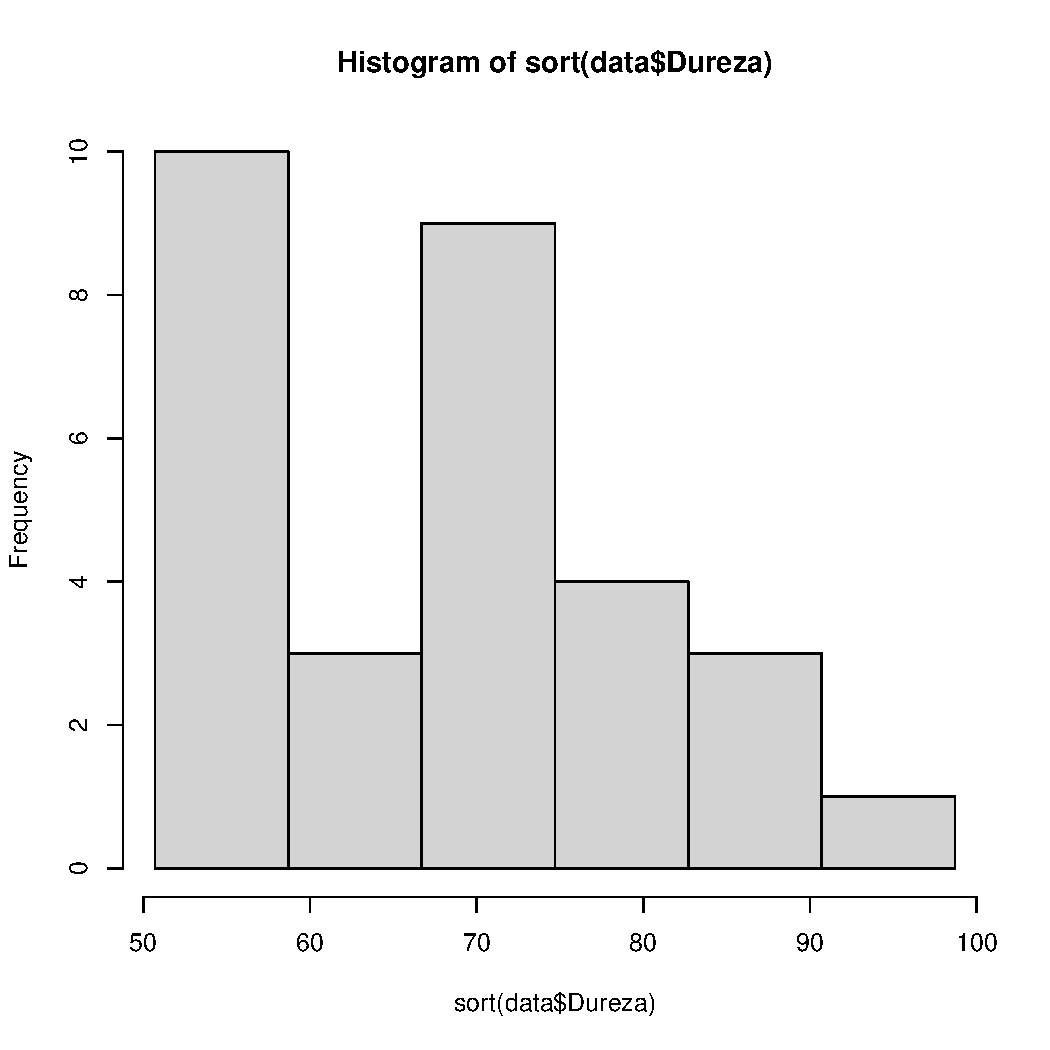
\includegraphics[width=8cm]{./../src/output/03212024_Output_HistogramaDurezaAluminio.pdf}
        \end{figure}
    \end{solution}
    \part Faça o box-plot dos dados. Existem outliers?
\end{parts}